%% The following is a directive for TeXShop to indicate the main file
%%!TEX root = diss.tex

\chapter{Introduction}
\label{ch:Introduction}

Storing and accessing information is one of the most important goals in computers. The data can be in many shapes and formats, and each of these  \acf{data instance} are collected into a repository. Open data is one such repository that contains a collection of data instances created and published by many individual authors, some of them government agencies. The rich repertoire of information in open data can be accessed by the general public without paying for the data. Along with the data instance itself, the repository also contains metadata for the data instance which can help someone to quickly understand what information is stored. Since each data instance stores different kinds of information, the metadata is very useful to describe and summarize the data stored, so that a user can browse a large number of data instances without too much effort trying to understand them. In general, the functions of metadata are explanation, summarization, and provenance \cite{10.1145/2845915}. The metadata can also help a user write queries on the data to answer his or her questions. The user or machine can easily perform searching and filtering that uses the metadata to group all the similar data into one place and access them together. At the same time, the metadata can aid machines to organize data, and track where the data came from, and link back to the original sources.

%%%%%%%%%%%%%%%%%%%%%%%%%%%%%%%%%%%%%%%%%%%%%%%%%%%%%%%%%%%%%%%%%%%%%%
\section{Definition of Metadata}
\label{sec:DefinitionOfMetadata}

Metadata is defined as “structured information about an information resource of any media type or format” \cite{Feltner2023Metadata}. There are three types of metadata as explained in \cite{Baca2008}: descriptive, administrative, and structural. Descriptive metadata tells what the data is about, administrative metadata stores information such as the intellectual property rights and use of information, and structural metadata helps relate different data together. Tags is one type of metadata used in open data and its role is both descriptive and structural. It comes in the form of a list of one or more text items (each item is a word or phrase).

\subsection{Tags as metadata}

Tags can provide context for the data which allows someone to understand what the data is about without looking into the data itself. This is a good property as discussed by \cite{Wilkinson2016FAIR}. With tags, the user can identify the intent of the data, determine its usefulness with respect to a given task, and take appropriate action. Tags can also help link different data instances together. If two data instances contain the same set of tags or overlap in many tags, then it is highly likely that the two data instances are similar and can be combined into a larger set of data.

%%%%%%%%%%%%%%%%%%%%%%%%%%%%%%%%%%%%%%%%%%%%%%%%%%%%%%%%%%%%%%%%%%%%%%
\section{Motivating example of tags}
\label{sec:MotivatingExampleOfTags}

We provide a motivating example from library studies, which emphasizes the usefulness of metadata. Journal articles are one type of data similar to open data; both are created and managed by different groups of authors. Each group manages a set of journal articles and is familiar with the contents of the articles, but the group is unfamiliar with articles managed by other groups. To aid a researcher to understand articles not managed by his or her group, metadata are tagged to each article. These metadata tags are usually created by the authors of the articles, and the purpose is to communicate with authors in other research groups who are interested in reading these articles. Once a researcher has read numerous articles with overlapping or similar tags, he or she is able to perform analysis, research, and generalize ideas from these articles.

%%%%%%%%%%%%%%%%%%%%%%%%%%%%%%%%%%%%%%%%%%%%%%%%%%%%%%%%%%%%%%%%%%%%%%
\section{The problems with anomalies in metadata}
\label{sec:TheProblemsWithAnomaliesInMetadata}

Open data was originally designed such that each data instance has complete and accurate data and metadata, which allows data in a repository to be more understandable and discoverable. However, in reality, many anomalies are present in the data and metadata. We focus on anomalies in the metadata. The metadata becomes less useful and misleading when it is incomplete, inaccurate, and heterogeneous.

\subsection{Incompleteness in metadata}

When the metadata does not contain complete information to summarize the contents of the data instance, it is insufficient to only look at the metadata to understand the underlying data. In the case of tags, the metadata for a data instance may contain some tags but it does not contain all of the tags needed to fully describe the data instance. The reason is that when an author creates tags for the data instance, he or she might only choose a few tags as metadata, and many other tags that could be useful are not included. When someone looks at the metadata of two related data instances, it might not be obvious that the two data instances contain related information because both of them only contain a few tags, and there are no overlaps between the two sets of tags.

\subsection{Inaccuracy in metadata}

Even if a data instance has rich metadata, the metadata may be inaccurate. For example, there may be spelling errors, typos, and formatting issues that prevents someone to interpret the metadata correctly. Even without errors, the tags may not be correctly chosen to describe the data instance.

\subsection{Heterogeneity in metadata}

There exists many types of heterogeneity in the metadata. In general, metadata items that resemble the same information might be represented differently across different data instances, and someone who do not know the different representations might not realize that the two metadata items are the same. Heterogeneities include mismatches in datatypes and differences in data granularities. With diverse data domains, each table is created for specific purposes, therefore the same data may have different meanings across different tables (and vice versa). This is known as semantic heterogeneity. A word can be represented using its synonyms, hypernyms, and acronyms, and resolving values that have the same meaning requires domain and technical expertise \cite{Halevy2005Why}.

In the case of metadata tags, many data instances share very similar data, but different data instances use different tags that are synonyms of each other. For example, the author of one journal article chooses a word as tag for the metadata, while an author of another journal article chooses a different word as tag for the metadata, without realizing that the two words are synonyms of each other. In the case of structured data instances (such as relational data), two attributes between two schemata represent the same information, but they use different attribute names.

A user may not find tags to be very useful when browsing or searching the tags due to the presence of heterogeneity. Someone who wants to read the two articles may only find one article relevant after looking at the metadata, because the tag words in the other article are unfamiliar to him or her. Without any technical expertise to resolve semantic heterogeneity, users need to spend more time manually perform searching, filtering, and browsing to find related tables. Once related tables are found, it is also difficult to understand how one table is related to another.

Due to incompleteness, inaccuracy, and heterogeneity in the metadata, a user may not be able to understand the data by only browsing its metadata, and a machine cannot use metadata to perform searching and filtering.

%%%%%%%%%%%%%%%%%%%%%%%%%%%%%%%%%%%%%%%%%%%%%%%%%%%%%%%%%%%%%%%%%%%%%%
\section{Scope of study and resources}
\label{sec:ScopeOfStudyAndResources}

We study how to improve metadata with the anomalies discussed in \autoref{sec:TheProblemsWithAnomaliesInMetadata}, we will discuss a number of methods and their effectiveness. We first limit the scope of our study. To make the problem simpler and easier to explain, we only study open data in the form of tables, and only seek to improve the quantity of metadata in the form of tags. Data instances in other forms such as XML, spatial data, and images are not studied. Metadata in the form of sentences, schema, and constraints also exist in open data, but we do not aim to improve them. A number of terminologies are defined as follows.

\subsection{Terminologies and definitions}

\begin{itemize}
\item Let a table be a two-dimensional matrix of values, where each column has a header. Let the header be the name of a column.
\item Let metadata tags be a list of text items, where each text item may be a word or a phrase, but the text item may not be a sentence, XML, or data mapping.
\item We also make a distinction between tags and topics, where a tag is a text item without any semantics, but a topic contains semantics such as a dictionary definition. A category is a tag, but there is fewer (likely only one) such tags per table.
\item Let a schema be a form of metadata, containing a list of mappings, where a header is mapped with a column. We call the header an attribute of the schema. In the notation A.b, A is the name of the schema, and b is the name of the attribute within A.
\item Let constraints be restrictions, for example, on the type of data stored in a column (enforcing all values in a column must be integer). Foreign keys is another type of constraint, that restricts which two columns can be joined.
\item Finally, let each data instance in open data contain only one table, and the metadata describing the table. We may use data instance and table interchangeably, depending on the context of use.
\end{itemize}

%%%%%%%%%%%%%%%%%%%%%%%%%%%%%%%%%%%%%%%%%%%%%%%%%%%%%%%%%%%%%%%%%%%%%%
\section{Open data case study}
\label{sec:OpenDataCaseStudy}

\begin{figure}
    \centering
    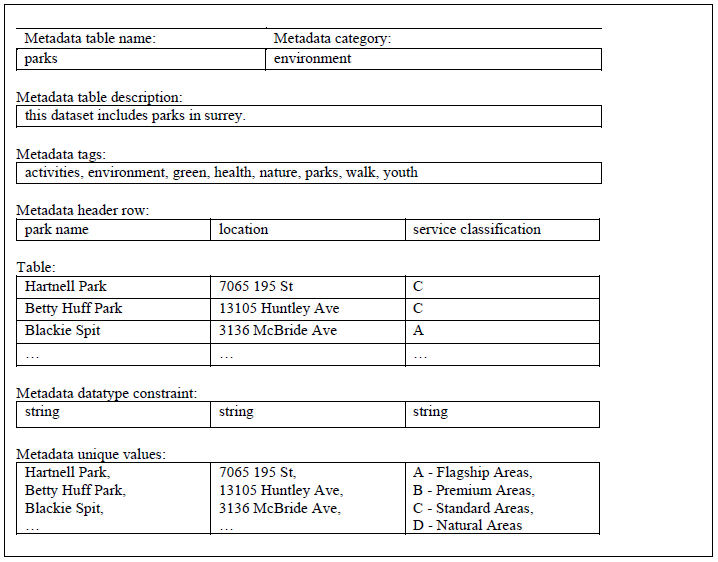
\includegraphics[width=5in]{figures/example-parks.png}
    \caption{Example data instance and metadata with table name parks}
    \label{fig:example-parks}
\end{figure}

We give examples of tables and metadata within an open data repository. We use City of Surrey Open Data1 as a case study. The metadata in this repository has many forms, such as the table name, the tags, the category the table belongs in, the header row of the tabular data, a paragraph in sentence form describing what information the table stores, the datatype constraint of each column, and the unique values in each column. Each metadata element either describes the entire table or a specific column of the table. \autoref{fig:example-parks} is an example of a table with its metadata. The table is the data instance containing data. The table name is parks. The table description informs that the table stores data for City of Surrey only. The category is environment; there may be other tables in the repository belonging in the same category. The tags list contains activities, environment, green, etc. The header row contains a list of column headers, such as the header park name for the first column of the table. For datatype constraint, the park name column is restricted to strings only, the other two columns are also restricted to strings. Values that are not the strings type do not appear in the column. The unique values contain example values of each column, such as `Hartnell Park' for park name.

Each metadata form is simplified to be a list of text items. For example, a table name is a list containing one text item (one or more words), while the header row is a list of headers, and each header is a text item. The table description is also a list containing one text item.

The data instance such as the one in \autoref{fig:example-parks} can be represented more concisely for different purposes. The representation of a schema is:

Parks(park name, location, service classification)

where Parks is the name of the table (and the name of the schema), and park name, location, service classification are the attributes of the schema.

Similarly, the tags of the data instance is represented as:

Parks: \{activities, environment, green, health, nature, parks, walk, youth\}

where activities, environment, green, health, nature, parks, walk, youth, are the tags in the metadata of Parks.

\autoref{fig:example-park-specimen-trees}, \autoref{fig:example-drainage-catch-basins}, \autoref{fig:example-park-screen-trees}, and \autoref{fig:example-park-structures} are other examples of a table with its metadata.

\begin{figure}
    \centering
    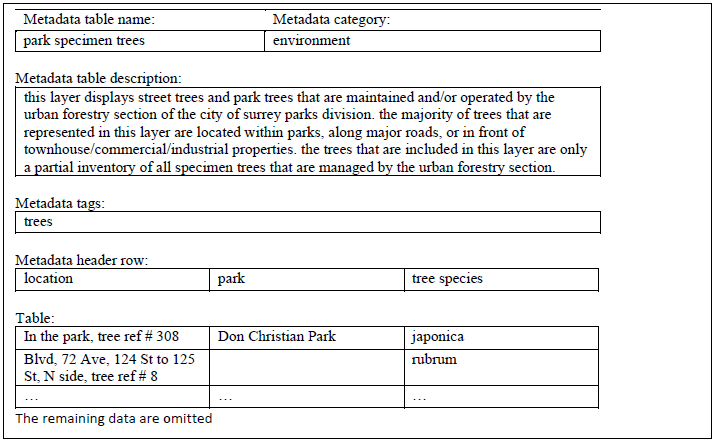
\includegraphics[width=5in]{figures/example-park-specimen-trees.png}
    \caption{Example data instance and metadata with table name park specimen trees}
    \label{fig:example-park-specimen-trees}
\end{figure}

\begin{figure}
    \centering
    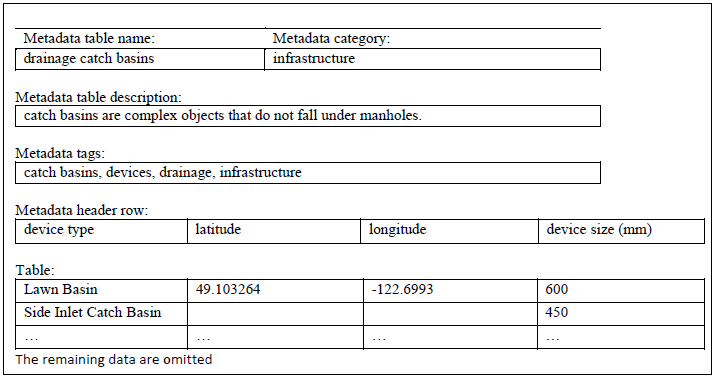
\includegraphics[width=5in]{figures/example-drainage-catch-basins.png}
    \caption{Example data instance and metadata with table name drainage catch basins}
    \label{fig:example-drainage-catch-basins}
\end{figure}

\begin{figure}
    \centering
    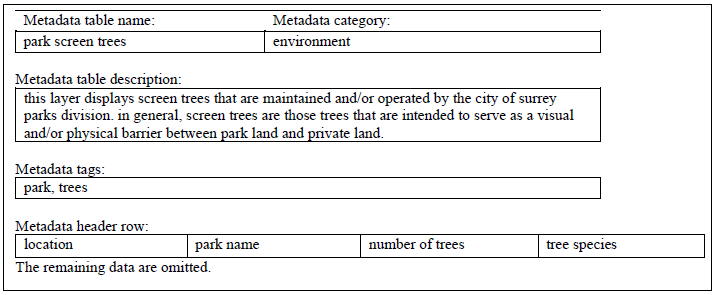
\includegraphics[width=5in]{figures/example-park-screen-trees.png}
    \caption{Example data instance and metadata with table name park screen trees}
    \label{fig:example-park-screen-trees}
\end{figure}

\begin{figure}
    \centering
    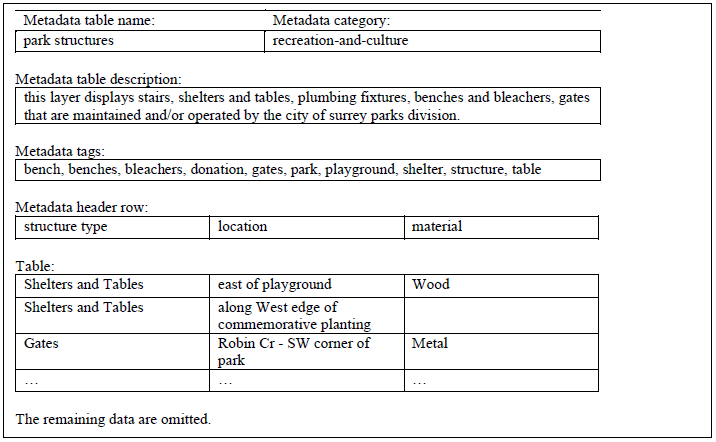
\includegraphics[width=5in]{figures/example-park-structures.png}
    \caption{Example data instance and metadata with table name park structures}
    \label{fig:example-park-structures}
\end{figure}

\subsection{Usefulness of header row in metadata}

We discuss what questions can be answered using the existing metadata in Surrey Open Data. When the table is available without any header row or any other metadata, it might not be clear what each of the values mean in the table. In \autoref{fig:example-parks}, the letters \textit{`C'} and \textit{`A'} in the third column could be interpreted in many ways. The letter might be the first letter of a word, or it might be a letter used for enumerating different classes. When the header row is present, each column is given more information to clarify what the column is about, but there is not enough information to interpret the values in the column. In \autoref{fig:example-parks}, the third column has the header service classification, which clarifies that the letters \textit{`C'} and \textit{`A'} are two service classes. But the header still does not inform what services \textit{`C'} and \textit{`A'} are.

If the user wants to join the two data instances in \autoref{fig:example-parks} and \autoref{fig:example-park-specimen-trees}, it is possible to join by \textit{location} since both tables have a column with the header \textit{location}. The user would find it much easier if they have access to the header rows when they first obtained the data instances. The header row allows the user to quickly find potential overlapping columns, and save time by not examining every column in the data instances. Although the header row itself is not informative enough to determine if two columns are joinable, it is still a good approximation. When the user sees two columns with a common header, the user is more likely to spend more time on the tables to investigate.

\subsection{Usefulness of unique values in metadata}

The \textit{unique values} contains all possible values in a column. If the values in the column are abbreviations or symbols, \textit{unique values} contains the full words for the abbreviations or symbols.

When the metadata is provided to each column, we can further decode the meaning of each value in a column. In \autoref{fig:example-parks}, values in the third column \textit{`C'} and \textit{`A'} are two classes of services, and the unique values decodes \textit{`C'} to \textit{`Standard Areas'} and \textit{`A'} to \textit{`Flagship Areas'}.

\subsection{Usefulness of tags in metadata}

Given some tables in a repository, the user would like to find out which tables are relevant to some tasks, and by using the metadata tags the user can quickly filter out irrelevant tables. In \autoref{fig:example-park-specimen-trees}, the table name is \textit{park specimen trees} and the only tag is \textit{trees}. In \autoref{fig:example-park-screen-trees}, the table name is \textit{park screen trees} and its tags are \textit{park} and \textit{trees}. Without looking into the values of the table instances, the user can quickly identify that both table instances contain some metadata about \textit{trees}, and if the user is interested in studying \textit{trees}, then both tables should be selected for further analysis. On the other hand, if the table name is drainage catch basins and the tags are \textit{devices} and \textit{infrastructure}, then the user should filter out the table immediately since the metadata does not seem to store any information about trees.

The idea of tag overlaps also applies to searching by machines. Using \autoref{fig:example-parks} and \autoref{fig:example-park-screen-trees} as an example, if the word \textit{park} is a search keyword, then both tables will be returned as results of the search, since both contain the word park in the metadata tags. But if the search is on park AND trees to search for information about trees in parks, then the metadata of the tables need to overlap in both park and trees in order to show up in the search result. Only the second table is returned in the search result because it overlaps in both tags. Note that it is evident from the table description that the word \textit{park} is interpreted as open green spaces.

%%%%%%%%%%%%%%%%%%%%%%%%%%%%%%%%%%%%%%%%%%%%%%%%%%%%%%%%%%%%%%%%%%%%%%
\section{Causes of anomalies in open data}
\label{sec:CausesOfAnomaliesInOpenData}

As discussed by \cite{10.1145/2845915}, present-day data management faces challenges in the aspects of volume, velocity, and variety. We will explain these challenges in the context of our study of open data and how they caused the anomalies in the data and metadata we discussed in \autoref{sec:TheProblemsWithAnomaliesInMetadata}.

Since the volume of some data collection is too large to be stored at one single location, and needs to be distributed to multiple locations, these data cannot be managed by one user. In open data repositories, there may be many attributes between schemata with complex relationships between them. However, it is difficult to discover these complex relationships when data are distributed.

Data grows at a very high velocity and is constantly changing, thus the users are required to constantly receive updates on the newest data. Managing the changing data also becomes difficult, and each of the tables becomes poor in quality because data values and metadata for tables are getting incomplete and inaccurate.

Due to the large volume of data and the rate that they are changing, it is inevitable that the data standards become out of sync where each individual user invents his or her own standards for maintaining the data that they have direct access to. Each user is able to maintain high quality for the data and metadata of their tables, but over time, the degree of heterogeneity between the data instances increases, which prevents one user to understand another user's data instance due to differences in constraints, data granularities, naming convention, and representation. If the different data instances did not belong in the same data domain initially, the difficulty to communicate information between the data instances can only be greater.

\subsection{Open data common anomalies}

In Surrey Open Data, tables show many data anomalies, and we will give examples to each anomaly. Looking at \autoref{fig:example-park-specimen-trees}, we see that there is a missing value in the second row in the column with header \textit{park}. When a table contains missing values, it is less likely for someone to correctly interpret the values in the table. When reading the table row by row, some rows may not make much sense due to missing some important values.

There are spelling errors or formatting inconsistencies in the table values. In \autoref{fig:example-park-specimen-trees}, values in the location column contain tree ref numbers, but some numbers are immediately preceded by a \verb+`#'+ symbol while others have a \verb+`#'+ followed by a space. Although the inconsistency is trivial to fix by hand for small table instances, it is more challenging if there are too many varieties of inconsistencies in many different tables and fixes can only be done programmatically. Many kinds of inconsistencies and spelling errors are difficult to detect, and if the fixes are done incorrectly, the values in the tables become even less interpretable.

Within each value, a user may find two or more kinds of information. In \autoref{fig:example-park-specimen-trees}, a value in the location column contains both the address as well as a reference number for the tree. To fix this issue, it is possible to move the reference number to a new column, and create a new header tree reference number for the new column.

Many abbreviations are used throughout the table instance in \autoref{fig:example-park-specimen-trees}. The word `ref' is the abbreviation for `reference', and `N' is the abbreviation for `North'. While humans are able to interpret these abbreviations by observing the context that they are used, a program may not be able to interpret them if it cannot access the context.

Semantic heterogeneity is prevalent in the tables. The column with header park name in \autoref{fig:example-parks} and the column with header park in \autoref{fig:example-park-specimen-trees} seem to store the same kind of information, the names of parks. However, without inspecting the values in the tables, it is less likely for the user to conclude that these two columns store the same kind of information. At the same time, in the location columns of \autoref{fig:example-parks} and \autoref{fig:example-park-specimen-trees}, abbreviations such as Blvd, St, and Ave all refer to names of roads for vehicles, but if the user does not already have the domain knowledge, these abbreviations do not share any similarities.

The anomalies discussed above also occur in the metadata, but since metadata aims to provide more useful information to make the table more understandable, there are less abbreviations, less spelling errors, and more concise representation of information \cite{Rahm2016Case}. However, metadata are more incomplete and heterogeneous due to the lack of effort creating them and maintaining them. In the case of \autoref{fig:example-park-specimen-trees}, the only tag in the metadata is trees, but tags such as park, species and urban should also be included to describe the table. The tag park has synonyms such as green and parkland, which should also be included in the metadata.

%%%%%%%%%%%%%%%%%%%%%%%%%%%%%%%%%%%%%%%%%%%%%%%%%%%%%%%%%%%%%%%%%%%%%%
\section{Scope of improving metadata}
\label{sec:ScopeOfImprovingMetadata}

There are many ways to improve the metadata and to fix the anomalies, but we are unable to discuss all of them. Our improvement is limited to the following scenario: a user is given a table he or she is familiar with, called a base table, and is given a number of tables in an open data repository. The user should be able to only look at the metadata to find all the related tables, and to get a sense of what data are stored in these tables. The user does not need to look at the contents in the tables to determine whether or not the two tables are similar.

It is often sufficient to show metadata that are related to the users goal. The user can understand the metadata more quickly because the unrelated metadata that could distract the user are not shown. If two tables overlap in a data domain of interest, then all metadata describing the data domain need to also overlap. If the two tables overlap in a data domain that is not related to a users goal, then overlaps in that data domain are not needed. Our work will be limited to improving metadata tags, we think tags are good summaries of the data contained in each table. Tags are machine-readable and can be processed by programs to perform keyword search or to compare between the tables.

To give an example, a user is interested in finding information about benches in parks, and finds one candidate table storing information about park structures of all types. In this table, there is a small portion of data storing benches in parks while the majority of data are about other information such as park gates and park tables. When we improve the metadata, we should only focus on improving metadata about benches, and ignore any additional metadata unrelated to benches. Tables containing information about benches must contain the tag bench as well as tags related to benches, while the improved tags does not need to contain tags unrelated to benches.

When the metadata does not contain tags, the user would have to manually summarize the contents of a table, which would require additional time. We therefore only seek to provide a basic summary with the metadata, so that the user can save some time. Similarly, in the presence of metadata anomalies, the user would need to compare tables to find out all possible tags related to the base table, and needs to study tables separately one by one to obtain a complete view of all the metadata.

\subsection{Idea: normalizing metadata}

We outline our general approach to improve the metadata tags of tables in an open data repository. If there are two tags describing the same information, the user would want to add both tags to the metadata of all the tables containing this information. We seek all such tags, and ensure each table contains all the tags describing the same information. We call this procedure normalization of metadata tags. In other words, a tag is added to all the relevant tables.

The user can then use any of these tags to perform search on the repository and obtain all the tables related to the base table. To achieve normalization, we need to describe how the metadata between the different tables are related, we use a mapping (between an attribute and a tag) called semantic labeling to capture the relatedness.

The relatedness then allows the tables reach a consensus on the representation of tags for all the tags that they share in common, so that overlap is maximized. Our approach is called augmentation of metadata. We look for existing tags in the related tables, and for all tables lacking these tags, we add the tags to these tables. We also examine the existing tags of a table to find other tags that can be shared between a group of related tables, and for the tables that do not already contain some of these tags, we add the tags to the tables. Augmentation of metadata is done in an iterative manner, where tags are gradually added to the metadata of each table in many iterations. This metadata augmentation procedure is done in a pay-as-you-go fashion, where only the related tables are augmented with tags, and only tags that relates to the base table are augmented.

\begin{figure}
    \centering
    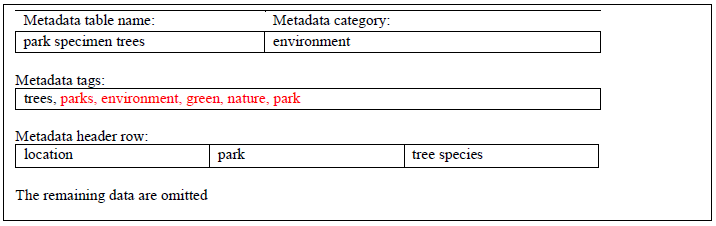
\includegraphics[width=5in]{figures/augmented-park-specimen-trees.png}
    \caption{Augmented tags of the table park specimen trees (shown in red)}
    \label{fig:augmented-park-specimen-trees}
\end{figure}

After the common representation of tags is found using normalization, tables with insufficient metadata is augmented with additional tags from a list of known tags. We show an example of the result of our automated metadata augmentation in \autoref{fig:augmented-park-specimen-trees}, using \autoref{fig:example-parks}, \autoref{fig:example-park-specimen-trees}, \autoref{fig:example-drainage-catch-basins}, \autoref{fig:example-park-screen-trees}, and \autoref{fig:example-park-structures} as our repository. In this example, additional tags for the park specimen trees table are added to the metadata, regardless of whether park specimen trees is the base table. The additional tags originate from other tables in the repository.

To overcome semantic heterogeneity, we perform semantic enrichment (attaching a dictionary definition to each word) of the metadata. We use a domain dictionary to assist us with listing all possible interpretations of a word. We use a technique called word sense disambiguation (probabilistically assign definition to each word) to find a correct interpretation of a word. We then use an algorithm called schema matching to create the semantic labeling of tables (by probabilistically matching between attributes and tags). The output of schema matching, called the correspondences, serves as the key intermediate for semantic labeling. To find the relatedness between tables, we adopt a table searching algorithm that relies on the semantic labeling to find the maximum tag overlaps between tables.

%%%%%%%%%%%%%%%%%%%%%%%%%%%%%%%%%%%%%%%%%%%%%%%%%%%%%%%%%%%%%%%%%%%%%%
\section{Problem Definition}
\label{sec:ProblemDefinition}

We will now define our problem that we have introduced in \autoref{sec:ScopeOfStudyAndResources} and \autoref{sec:ScopeOfImprovingMetadata}. The input to our problem is a set of data instances, each containing a table, a metadata schema for the table, and a list of metadata text items describing the data instance. Each table contains a header row, and there is a column header for each table column. The text items may or may not be able to describe the table.

\subsection{Inputs and outputs}

More formally, let a data instance, s, consist of:
\begin{itemize}
\item A Table Ts , where Ts contains a header row that consists of column headers, but no type information
\item Let As be the attributes within the schema of Ts , where each attribute provides constraints for a header. We denote the attribute for the ith header in the header row of table Ts as Asi
\item Ls , a list of text items describing the contents of s , where Lsj is the jth text item in Ls
\end{itemize}
We take as input to our problem:
\begin{itemize}
\item A base data instance sq to be compared with other data instances
\item a set of $k$ data instances, D, from unknown domains, which could be related to the sq . The correspondences between attributes of these data instances are unavailable. The semantic labeling is also unavailable.
\item A domain dictionary W , that can provide the semantics for values in Ts , As , and Ls
\end{itemize}
The outputs are:
\begin{itemize}
\item A set of data instances l  D related to sq, where l . k
\item A augmented list of L'sq such that L'sq more accurately describes the contents of sq
\item l augmented lists of L's such that L's more accurately describes the contents of s  D than Ls
\end{itemize}

\subsection{Assumptions}

Under the following assumptions, our solutions can be correctly implemented:

\begin{enumerate}
\item Each table contains a list of likely incomplete text items (metadata tags) describing the contents of the data instance. The list can be empty
\item The authors made an attempt at creating the metadata, it was not generated without inspection, therefore we trust the provided metadata
\item The goal of augmenting metadata tags for a table is for the user to get approximate answers quickly, but not precise answers. That is, metadata tags are augmented in a pay-as-you-go fashion
\item The user already knows what kinds of metadata is useful and interesting to look at, therefore we just have to augment tags that the user needs
\item All attributes in one schema are independent of one another. This assumption may not be true, but it is plausible and allows us to simplify our problem
\item The set of all topics in the repository are the only topics used for augmenting tables, that is, we do not create new topics that did not already exist in the repository. This assumption reduces a lot of uncertainty in our evaluations	
\end{enumerate}

%%%%%%%%%%%%%%%%%%%%%%%%%%%%%%%%%%%%%%%%%%%%%%%%%%%%%%%%%%%%%%%%%%%%%%
\section{Contributions}
\label{sec:Contributions}

The contributions we make in this thesis are the following:
\begin{enumerate}
\item We give a different perspective to the problem of augmenting tags in tables with incomplete metadata. We proposed an iterative approach, where given a base table with incomplete metadata, find other tables in the repository similar to the base table, and then iteratively find as much overlap between all related tables as possible.
\item We give a detailed explanation of why high-quality metadata can reveal new information to the user and how it can help organize existing data in a repository. We outlined that it is easy for users to navigate a repository, perform filter and search, and understand data and metadata of tables without looking at the values in the tables. Metadata tags also allows more automation in that they increase precision and recall for machine operations.
\item We discuss a number of techniques used to solve other problem, and we explain how these techniques can be applied to our problem.	
\end{enumerate}

The rest of this thesis is presented as follows. In \autoref{ch:RelatedWork}, we discuss a number of related fields of study and point out the strengths and weaknesses in solving our problem. In \autoref{ch:Preliminaries}, we provide detailed explanations of techniques that we used in our approach to augment metadata. In \autoref{ch:Solutions}, we discuss our proposed approaches as well as baseline approaches in solving the metadata augmentation problem. In \autoref{ch:Implementations}, we discuss how we implemented our approaches as well as the evaluations of our approaches. In \autoref{ch:Discussions}, we provide discussions of metadata augmentation and how it plays a role in data management research. We conclude in \autoref{ch:Conclusion}.
\endinput